\documentclass[11pt,a4paper,draft]{article}
\usepackage[english]{babel} % Using babel for hyphenation
\usepackage{lmodern} % Changing the font
\usepackage[utf8]{inputenc}
\usepackage[T1]{fontenc}

\usepackage{csquotes}
\usepackage[sortcites=true,sorting=nyt,backend=biber]{biblatex}
\addbibresource{bibliography.bib}


\usepackage[colorlinks=true]{hyperref}
\usepackage{cleveref}

%\usepackage[moderate]{savetrees} % [subtle/moderate/extreme] really compact writing
\usepackage{framed}
\usepackage{tcolorbox}
\tcbuselibrary{hooks}
\usepackage[parfill]{parskip} % Removes indents
\usepackage{amsmath} % Environment, symbols etc...
\usepackage{amssymb}
\usepackage{float} % Fixing figure locations
\usepackage{multirow} % For nice tables
%\usepackage{wasysym} % Astrological symbols
\usepackage{graphicx} % For pictures etc...
\usepackage{enumitem} % Points/lists
\usepackage{physics} % Typesetting of mathematical physics examples: 
                     % \bra{}, \ket{}, expval{}
\usepackage{url}


\usepackage{caption}
\usepackage{subcaption}

\definecolor{red}{RGB}{255,10,10}

% To include code(-snippets) with æøå
\usepackage{listings}
\lstset{
language=c++,
showspaces=false,
showstringspaces=false,
frame=l,
}

\tolerance = 5000 % Bedre tekst
\hbadness = \tolerance
\pretolerance = 2000

\numberwithin{equation}{section}

\newcommand{\conj}[1]{#1^*}
\newcommand{\ve}[1]{\mathbf{#1}} % Vektorer i bold
\let\oldhat\hat
\renewcommand{\hat}[1]{\oldhat{#1}}
\newcommand{\trans}[1]{#1^\top}
\newcommand{\herm}[1]{#1^\dagger}

\newcommand{\Real}{\mathbb{R}}
\newcommand{\bigO}[1]{\mathcal{O}\left( #1 \right)}


\newcounter{algcounter}
\renewcommand{\thealgcounter}{\Roman{algcounter}}

\newenvironment{algorithm}{%
\refstepcounter{algcounter}
\begin{tcolorbox}
\centerline{Algorithm \thealgcounter}\vspace{2mm}
}
{\end{tcolorbox}}

\newcommand{\figurewidth}{.85\textwidth}

\title{FYS3150/4150\\Computational Physics\\Project 5}
\author{Magnus Ulimoen \& Krister Stræte Karlsen\\
Candidate numbers 33 \& 63}
\date{\today}

\begin{document}
\tcbset{before app=\parfillskip0pt}
\maketitle

\begin{abstract}
This project studies the diffusion equations using both finite difference methods and monte carlo methods. Accuracy and stability for the methods will be compared, and a practical application of transporting signals in the brain via diffusion will be briefly introduced. 
\end{abstract}

The program used is hosted on Github, at 
\url{https://github.com/mulimoen/FYS3150CompPhy} under project 5.

\section{Introduction}
The dominant way of transporting signals between nerve cells in the brain is by means of diffusion of neurotransmitters across the synaptic cleft separating the cell membranes of the two cells. A simple model for this phenomenon is a one dimensional diffusion equation (see figure 1 for schematic drawing of the process). 

\begin{figure}[H]
\centering
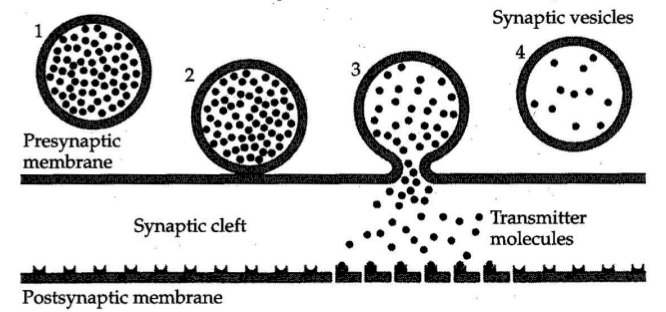
\includegraphics[scale=0.15]{pics/SynapticVesicle.png}
\caption{Illustration of the process of vesicle release from the axon
terminal and release of transmitter molecules into the synaptic cleft.
(From \cite{thompson2000brain}.)}
\end{figure}

The diffusion equation will be solved using three finite difference schemes, explicit \emph{Forward-Euler}, implicit \emph{Backward-Euler} and implicit \emph{Crank-Nicholson}. These methods will be compared with respect to stability and accuracy. Monte carlo methods, following the lines of \cite{farnell2005monte}, will also be used for solving the diffusion problem.

\section{Mathematical problem}
A mathematical formulation of this problem is a diffusion equation on the form
\begin{gather}
\frac{\partial u}{\partial t} = D\nabla^2u
\end{gather}
Where $D$ is a constant determining how ''solid'' the fluid which is 
diffused through is. Our problem is one-dimensional and has conditions on 
the boundaries.
\subsection{Boundary conditions}
The domain is $x \in [0, d]$ with boundary and initial conditions
\begin{align}
u(x,0) &= 0\\
u(0,t) &= u_0\\
u(d,t) &= 0.
\end{align}

\subsection{Scaling}
To make this problem more general and easier to solve we introduce 
scaling of the dimensions. This gives dimensionless parameters which 
are easily adapted to all sorts of diffusion problems.

Length scaling
\begin{equation}
\tilde{x} = \frac{x}{d}
\end{equation}
Time scaling
\begin{equation}
\tilde{t} = t\frac{D}{d^2}
\end{equation}
Amplitude scaling
\begin{equation}
\tilde{u}(x,t) = \frac{u(x,t)}{u_0}
\end{equation}
Our equation then takes the simple form
\begin{gather}
\frac{\partial \tilde{u}}{\partial \tilde{t}}
= \frac{\partial \tilde{u}^2}{\partial \tilde{x}^2}\\
0 \le \tilde{x} \le 1\\
\tilde{u}(0,\tilde{t})
= 1, \quad \tilde{u}(1,\tilde{t}) = 0, \quad \tilde{u}(\tilde{x}, 0 ) = 0
\end{gather}
In the next sections we will drop the tilde and work with the 
dimensionless parameters.

\subsection{Analytical solution}
In the steady state we must have
\begin{gather}
\frac{\partial^2 u_s}{\partial x^2} = 0
\end{gather}
This has the solution
\begin{gather}
u_s(x) = Ax + b\\
u_s(0) \implies b = 1, \quad
u_s(1) \implies A = -1\\
u_s(x) = 1-x \label{eq:u_steady}
\end{gather}
Defining the new non-steady solution
\begin{gather}
v(x,t) = u(x,t) - u_s(x)\\
v(x,0) = -u_s(x)\\
v(0,t) = v(1, t) = 0
\end{gather}
To solve this equation we assume that it is on the separable form
\begin{gather}
v(x,t) = X(x)T(t)
\end{gather}
And so
\begin{gather}
\frac{\partial^2 X(x)T(t)}{\partial x^2}
= \frac{\partial X(x)T(t)}{\partial t}\\
\frac{1}{X(x)}\frac{\partial^2 X(x)}{\partial x^2}
 = \frac{1}{T(t)}\frac{\partial T(t)}{\partial t} = C
 \label{eq:coupled_constant}
\end{gather}
The solution to these two equations are 
\begin{gather}
X(x) = \sin(\pi kx) \lor \cos(\pi kx)\\
T(t) = e^{\pm at}
\end{gather}
Since $T(t)$ can not grow to infinity, only the solution with a 
negative exponential is allowed. Using the boundary conditions at 
$x=0$, we see that the cosine solution is not possible.
The relation on the other boundary gives 
\begin{gather}
\pi k = n\pi
\end{gather}
with n as an integer. $k$ is quantized as an integer. The full solution 
is the superposition of all the solutions,
\begin{gather}
v(x,t) = \sum_{n=1}^\infty c_k \sin(\pi kx)e^{-(k\pi)^2t}
\end{gather}
To determine $c_k$ we use the Fourier expansion of the initial 
state \eqref{eq:u_steady}, 
%(this is from Rottman page 122, Fourier-rekker)
\begin{gather}
\frac{\pi - x}{2} = \sum_{n=1}^\infty \frac{\sin(nx)}{n}
\end{gather}
Which gives
\begin{gather}
x-1 = -\frac{2}{\pi}\sum_{k=1}^\infty \frac{\sin\pi kx}{k}
\end{gather}
And the Fourier constants
\begin{gather}
c_k = -\frac{2}{\pi k}
\end{gather}
And the analytical solution
\begin{gather}
v(x,t) = -\sum_{k=1}^\infty \frac{2}{\pi k}\sin(k\pi x)e^{-(k\pi)^2t}
\end{gather}



\section{Finite difference methods}

Let the spatial domain $x \in [0,d]$ be sampled at $N+1$ points, $x_0,x_1,..,x_i,..,x_L$ and the time be discretised as $t_0,t_1,..,t_n,..,t_N$. Then we denote the solution, $u(x_i,t_n)$, as $u_i^n$.  

\subsection{Schemes}

\subsubsection{Explicit Euler}
Using a forward discretisation of the time-derivative we obtain the following finite difference approximation of the diffusion equation:
\begin{align}
\frac{u_{i}^{n+1}-u_{i}^{n}}{\Delta t} = \frac{u_{i-1}^{n}-2u_{i}^{n}+u_{i+1}^{n}}{\Delta x^2}
\end{align}
Solved for $u_{i}^{n+1}$ the explicit Euler scheme is recovered:
\begin{gather}
u_i^{n+1} = u_i^n + \frac{\Delta t}{\Delta x^2}\left(
u_{i+1}^n - 2u_i^n + u_{i-1}^n
\right)
\end{gather}
Written in a matrix equation with boundary conditions (the notation 
is explained in \ref{subsubsec:implicit_euler})
\begin{gather}
\mathbf{u^{n+1}} = 
\begin{pmatrix}
1 & 0 & 0 & 0 & \cdots\\
\alpha & 1 - 2\alpha & \alpha & 0 & \cdots\\
0 & \alpha & 1-2\alpha & \alpha & \cdots\\
\cdots & \cdots & \ddots & \ddots& \\
&&& 0 & 1
\end{pmatrix} \mathbf{u^n}
\end{gather}


\subsubsection{Implicit Euler}
\label{subsubsec:implicit_euler}

Using a backward discretisation of the time-derivative we obtain the following finite difference approximation of (2.11):
\begin{align}
\frac{u_{i}^{n}-u_{i}^{n-1}}{\Delta t} = \frac{u_{i-1}^{n}-2u_{i}^{n}+u_{i+1}^{n}}{\Delta x^2}
\end{align}
Moving all unknowns to the left hand side and defining $\alpha = \frac{\Delta t}{\Delta x^2}$ we get
\begin{align*}
-\alpha u_{i-1}^n + (1+2\alpha)u_i^n - \alpha u_{i+1}^n = u_i^{n-1}. 
\end{align*}
Let's say we have only five spatial mesh points and Dirichlet boundary conditions, $u(0)=D_0$ and $u(d)=D_1$ , then all the equations reads
\begin{align*}
u_0^n &= D_0 \\
-\alpha u_{0}^n + (1+2\alpha)u_1^n - \alpha u_{2}^n &= u_1^{n-1} \\
-\alpha u_{1}^n + (1+2\alpha)u_2^n - \alpha u_{3}^n &= u_2^{n-1} \\
-\alpha u_{2}^n + (1+2\alpha)u_3^n - \alpha u_{4}^n &= u_3^{n-1} \\
u_L^n &= D_1 
\end{align*}
This now should be recognized as a matrix system on the from, $Au=b$ for 
\begin{align}
\begin{pmatrix} 1 & 0 & \dots   & \dots         & 0 \\
                -\alpha & 1+2\alpha & -\alpha & 0           &0 \\
        \dots  & \ddots & \ddots & \ddots         & \dots\\
 0   & \dots &  -\alpha & 1+2\alpha & -\alpha \\
 0   & \dots & \dots & \dots    &  1
             \end{pmatrix}
\begin{pmatrix} D_0 \\
      u_1^{n-1} \\
      u_2^{n-1}\\ \dots\\ u_{L-1}^{n-1}\\
      D_1
\end{pmatrix} 
=  \begin{pmatrix} u_0^n \\
                   u_1^n  \\
           \dots\\ \dots\\ \dots\\
                   u_L^n 
             \end{pmatrix} 
\end{align} 

\subsubsection{Crank-Nicholson}
This scheme uses a time-centered difference at $u_i^{n+1/2}$, which means that also the spatial derivative must be evaluated at $t_{n+1/2}$. To get such an approximation one can use an arithmetic mean, $u'(t_{n+1/2}) \simeq \frac{1}{2}(u'(t_{n}) + u'(t_{n+1}))$. The full discretisation then reads 
\begin{gather}
\frac{u_{i}^{n+1}-u_{i}^{n}}{\Delta t} = \frac{1}{2} \left( \frac{u_{i+1}^{n} -2 u_{i}^{n}+u_{i-1}^{n}}{\Delta x^2} + \frac{u_{i+1}^{n+1} -2u_{i}^{n+1}+u_{i-1}^{n+1} }{\Delta x} \right)
\end{gather}


\begin{gather}
u_i^{n+1} = u_i^n + \frac{\Delta t}{2\Delta x^2}\left(
u_{i+1}^n - 2u_i^n + u_{i-1}^n + u_{i+1}^{n+1} - 2u_i^{n+1} + u_{i-1}^{n+1}
\right)
\end{gather}
In a matrix equation it takes the form
\begin{gather}
u^{n+1} = u^n + \frac{\Delta t}{2\Delta x^2}
\begin{pmatrix}
-2 & 1 & 0\\
1 & -2 & 1\\
0 & 1 & -2
\end{pmatrix} u^n
 + \frac{\Delta t}{2\Delta x^2}
\begin{pmatrix}
-2 & 1 & 0\\
1 & -2 & 1\\
0 & 1 & -2
\end{pmatrix}u^{n+1}\\
\begin{pmatrix}
1 & 0 & 0 & 0\\
-\frac{\alpha}{2} & 1 + \alpha & -\frac{\alpha}{2} & 0\\
0 & -\frac{\alpha}{2} & 1 + \alpha & -\frac{\alpha}{2}\\
0 & & \ddots\\
&&& 1
\end{pmatrix}
u^{n+1} = 
\begin{pmatrix}
1 & 0 & 0 & 0\\
\frac{\alpha}{2} & 1 - \alpha & \frac{\alpha}{2} &  0\\
0 & \frac{\alpha}{2} & 1 - \alpha & \frac{\alpha}{2}\\
&& \ddots\\
&&&1
\end{pmatrix}u^n
\end{gather}


\subsubsection{Specialisation to our problem}

If we consider our problem with ends equal to zero, the schemes can 
be reduced to a sub-matrix with the corners equal to zero, and is therefore
not required to reach the solution. All the three schemes can be written 
with the use of the matrix
\begin{gather}
A = 
\begin{pmatrix}
a & b & 0 & \cdots\\
b & a & b & \cdots\\
&&\ddots & \ddots\\
&&0& b& a & b\\
&&&&b&a
\end{pmatrix}
\label{eq:matrixA}
\end{gather}

\subsubsection{The $\theta-$scheme}

\subsection{Truncation error analysis}

To investigate the truncation error in the schemes we look into the approximations we have made deriving them. In order to do that we need the following Taylor series:
\begin{equation}
u(a+h) = u(a) +hu'(a)+O(h^2)
\end{equation}
\begin{equation}
u(a+h) = u(a) +hu'(a)+\frac{1}{2}h^2 u''(a) +O(h^3)
\end{equation}
\begin{equation}
u(a+h/2) = u(a) +\frac{h}{2}u'(a) + \frac{1}{2} \left( \frac{h}{2} \right)^2 u''(a) + O(h^3)
\end{equation}

\subsubsection{Explicit Euler}
The forward time-derivative is obtained by solving (??) for $u'(a)$, with $a=t$ and $h=\Delta t$
\begin{equation}
\frac{u(t+\Delta t)-u(t)}{\Delta t} = u'(t)+O(\Delta t).
\end{equation}  
Having to divide by $h$ we get an truncation error of $O(h)$ in time.

The second derivative with respect to space is obtained by adding (??), with $a=x$,  $h=\Delta x$ and 
$a=x$,  $h= -\Delta x$ and solving for $u''(x)$:
\begin{equation}
\frac{u(x+\Delta x)-2u(x)+u(x-\Delta x)}{\Delta x^2} = u''(x)+O(\Delta x^2).
\end{equation}  

Using these approximations we have that the truncation error of the Forward Euler scheme is of magnitude $O(\Delta x^2)+O(\Delta t)$.  

\subsubsection{Implicit Euler}
The error analysis for this scheme is the same as for the forward scheme. One can just set $h=- \Delta t$
instead of $h=\Delta t$ and hence recover the same truncation error, $O(\Delta x^2)+O(\Delta t)$. However, it is "cheaper", computational wise, to obtain more accuracy using this scheme for stability reasons(discussed in section (??)). 

\subsubsection{Crank-Nicholson}
To ensure better accuracy a center derivative in time can be used as well. By letting $a=t+\Delta t/2$, $h=\Delta t$ and subtracting $a=t-\Delta t/2$, $h=-\Delta t$ for the series (??) we get the following center time-derivative:
\begin{equation}
\frac{u(t + \Delta t)-u(t)}{\Delta t} = u'(t+\Delta t) + O(\Delta t^2)
\end{equation}
Having evaluated the time-derivative in $t+\Delta t$ we must evaluate the spatial-derivative in between time-points. This can be done by using an arithmetic mean of the two closest time-points
\begin{align*}
u(t+\Delta t/2) \simeq \frac{1}{2}(u(t)+u(t+\Delta t)).
\end{align*}
Using the approximation above combined with the expression for the second order derivative we get a truncation error of $O(\Delta x^2)+O(\Delta t^2)$ for the Crank-Nicholson scheme.

\subsection{Stability analysis}

The key to our stability analysis is to investigate how the numerical solution grows(or in the case of diffusion; decays) compared to the analytical. This will be done by using the known analytical solution on the form:
\begin{equation}
u(x,t) = T(t)e^{ik \pi x} = e^{-(k\pi)^t}e^{ik \pi x}
\end{equation}
The solution consists of a periodic wave component, and a component decaying in time, $T(t)=e^{-(k\pi)^t}$. We will define a discrete solution on the form
\begin{equation}
v^n_i = A^n e^{ik \pi x_i}
\end{equation}
and insert it into the different discrete equations(schemes) and see what restrictions this puts on $\Delta x$ and $\Delta t$ (\emph{i} sub-script is discrete spatial position, not the imaginary unit as in the wave component).

This form of analysis is known as \emph{Von Neumann's stability analysis}.

\subsubsection{Explicit Euler}

By inserting the discrete solution, $v^n_i$, into the explicit Euler scheme we get
\begin{align*}
\frac{A^{n+1}-A^{n}}{\Delta t} e^{ik \pi x_i} = \frac{e^{ik \pi x_{i+1}} -2e^{ik \pi x_i} + e^{ik \pi x_{i-1}}}{\Delta x^2} A^n.
\end{align*}
If we now use the fact that $x_i = i\Delta x$ and divide both sides by $A^n e^{ik \pi x_i}$ we obtain the simpler equation
\begin{align*}
\frac{A-1}{\Delta t} = \frac{e^{ik \pi \Delta x} -2 + e^{-ik \pi \Delta x}}{\Delta x^2} = -\frac{4}{\Delta x^2}sin^2\left(k\pi \frac{\Delta x}{2}\right)
\end{align*}
which solved for $A$ gives
\begin{align*}
A=1-\frac{4\Delta t}{\Delta x^2}sin^2\left(k\pi \frac{\Delta x}{2}\right).
\end{align*}
Now, since $T(0)=1$ and $T(t)$ is decaying we must have that $|A| \leq 1$, that is, from the expression above, 
\begin{align*}
\abs{ \frac{4\Delta t}{\Delta x^2}sin^2\left(k\pi \frac{\Delta x}{2}\right)} \leq 2
\end{align*} 
which is satisfied for $\frac{\Delta t}{\Delta x^2} \leq \frac{1}{2}$. The scheme is so called \emph{conditionally stable}.

\subsubsection{Implicit Euler}
We follow the same reasoning and procedure as for explicit Euler and start by inserting the discrete solution, $v^n_i$, into the scheme:
\begin{align*}
\frac{A^{n}-A^{n-1}}{\Delta t} e^{ik \pi x_i} = \frac{e^{ik \pi x_{i+1}} -2e^{ik \pi x_i} + e^{ik \pi x_{i-1}}}{\Delta x^2} A^n.
\end{align*}
If we now use the fact that $x_i = i\Delta x$ and divide both sides by $A^n e^{ik \pi x_i}$ we obtain the simpler equation
\begin{align*}
\frac{1-A^{-1}}{\Delta t} = \frac{e^{ik \pi \Delta x} -2 + e^{-ik \pi \Delta x}}{\Delta x^2} = -\frac{4}{\Delta x^2}sin^2\left(k\pi \frac{\Delta x}{2}\right)
\end{align*}
which solved for $A$ gives
\begin{align*}
A=\left( \frac{4\Delta t}{\Delta x^2}sin^2\left(k\pi \frac{\Delta x}{2}\right)-1 \right)^{-1}.
\end{align*}
Again we require that $|A| \leq 1$, which this time puts no restrictions on the $\Delta t/ \Delta x^2$ relationship. This is therefore a so called \emph{unconditionally stable} scheme.


\subsubsection{Crank-Nicholson}
To quote the cult television classic \emph{Dinner for one}:  \emph{"Same procedure as every year, James!}

Inserting  $v^n_i$, into the Crank-Nicholson scheme
\begin{align*}
\frac{A^{n+1} - A^{n}}{\Delta t} e^{ik \pi x_i} = \frac{1}{2} \left( \frac{e^{ik \pi x_{i+1}}-2e^{ik \pi x_{i}} + e^{ik \pi x_{i-1}}}{\Delta x^2} (A^n + A^{n+1})  \right)
\end{align*}
which can be written 
\begin{align*}
\frac{A-1}{\Delta t} &= \frac{1}{2} \left( \frac{e^{ik \pi \Delta x} -2 + e^{-ik \pi \Delta x}}{\Delta x^2} (1 + A) \right) \\
&= \frac{1}{2} \left( -\frac{4}{\Delta x^2}sin^2\left(k\pi \frac{\Delta x}{2}\right)(1 + A) \right).
\end{align*}
Solving this equation for $A$
\begin{align*}
A = \frac{1-\frac{2\Delta t}{\Delta x^2}sin^2\left(k\pi \frac{\Delta x}{2}\right)}{1+\frac{2\Delta t}{\Delta x^2}sin^2\left(k\pi \frac{\Delta x}{2}\right)}
\end{align*}
we see that $|A| \leq 1$ is fulfilled, and the scheme is  \emph{unconditionally stable}.

\subsection{Convergence rate}

Convergence rates are important when verifying the implementation of numerical schemes. If we manage to recover the convergence rates expected from the truncation error analysis there is a good chance that our program is running correctly.

 One should expect that the error $E$ in the numerical solution is reduced if the mesh is refined. More specifically, many numerical methods obey a power-law relation between $E$ and step length $h$
\begin{align*}
E=Ch^r,
\end{align*}
where $C$ is just some constant and $r$ is known as the convergence rate.  

For some chosen time-level the error will be computed according to 
\begin{equation}
E = \sqrt{\frac{1}{N+1} \sum_{i=0}^{N} (u_{e(i)}-u_{i})^2}
\end{equation}
which is the \emph{discrete L2-norm}. 

The convergence rate can then be computed as
\begin{align*}
r_i = \frac{log(E_{i-1}/E_i)}{log(h_{i-1}/ h_i)}
\end{align*}
for a number of different numerical simulations, $i=1,2,3..$ using different $h_i=\Delta t^k = \Delta x^2 $, with $k=1$ for explicit and implicit Euler and $k=2$ for Crank-Nicholson. These choices are based on the truncation error analysis.  

\section{Monte Carlo methods}

The diffusion equation has close ties with random walk. If we let a 
particle only be able to move to the right or the left, we should obtain
the solution to the diffusion equation when the number of samplings 
increases.

The methods used here are based on \cite{farnell2005monte}. This gives 
the standard displacement for a particle in one dimension 
as $l_0 = \sqrt{2D\Delta t}$.

\subsection{Equal step length}
Letting the particles move on a solid lattice we can place them as 
numbers in a vector, where each number is equal to the number of 
particles in that position. Then we can choose the number of particles
from  each bin that is going to the right, and letting the rest go
to the left. 
How many going to right is decided by a binomial distribution.

\subsection{Unequal step length}
The other method that we are exploring is letting all the particles 
walk a distance $L_0\zeta$ with $\zeta$ as a number from a normal 
distribution with mean 1. This should more closely resemble real
particles, as they show a somewhat equal resemblance to the velocity 
distribution.


\subsection{Choice of random number generator}

For the MC-methods the Mersenne Twister from the \emph{<random>}
header in the standard library in C++ is used. This should give numbers 
with a suitable entropy and period.


\section{Implementation}


\subsection{Sparse matrix}
The matrices encountered in the solvers are very sparse, with the same 
diagonal element and off-diagonals. In order to maximize performance 
we implement solvers for the necessary operations.

The schemes used can all be represented as a multiplication with 
a matrix on the form of \eqref{eq:matrixA}. The matrix multiplication is 
straight forward to implement, and the inverse matrix multiplication uses
the same method as in project 1, which is in the Github repository.

\subsection{Finite difference schemes}

\subsubsection{Explicit Euler}
\begin{algorithm}
\begin{enumerate}[label=\bfseries \arabic*)]
\item Calculate
\begin{gather*}
\alpha = \frac{\Delta t}{\Delta x^2}\\
a = 1 - \alpha\\
b = \alpha
\end{gather*}
\item Multiply $u^n$ with the matrix A, \eqref{eq:matrixA}
\item Repeat for the next time-step
\end{enumerate}
\end{algorithm}

\subsubsection{Implicit Euler}
\begin{algorithm}
\begin{enumerate}[label=\bfseries \arabic*)]
\item Calculate
\begin{gather*}
\alpha = \frac{\Delta t}{\Delta x^2}\\
a = 1 + \alpha\\
b = -\alpha
\end{gather*}
\item Solve the matrix equation $d = Au$ with A as \eqref{eq:matrixA},
and $d$ as $u^n$ using TDMA. The solution is $u^{n+1}$

\item Repeat for the next time-step
\end{enumerate}
\end{algorithm}

\subsubsection{Crank-Nicholson}
\begin{algorithm}
\begin{enumerate}[label=\bfseries \arabic*)]
\item Calculate
\begin{align*}
\alpha = \frac{\Delta t}{\Delta x^2}\\
a_1 &= 1 - \frac{1}{2}\alpha, \quad
b_1 = \frac{1}{2}\alpha\\
a_2 &= 1 + \frac{1}{2}\alpha, \quad
b_2 =-\frac{1}{2}\alpha
\end{align*}

\item Do a matrix multiplication with $u^n$ and $A_1$, where $A_1$ has 
the entries $a_1$ and $b_1$ on the form of \eqref{eq:matrixA}.

\item Do an inverse matrix multiplication with $A_2$, where $A_2$ has 
the entries $a_2$ and $b_2$

\item Repeat for the next time-step

\end{enumerate}
\end{algorithm}

\subsection{Monte Carlo}
The Monte Carlo method with equal steps is very simple to program, and 
is therefore just included in the source code. The algorithm for 
unequal step length
\begin{algorithm}
\begin{enumerate}[label=\bfseries \arabic*)]
\item Set up the lattice with all the particles in bin 0
\item Let each particle move a length $L_0\zeta$ with $\zeta$ drawn
from a normal distribution with mean 0, and $\sigma = 1$
\item Clean up particles outside $(0,1)$
\item Repeat 2)-3) for the next time step
\item Bin up all the particles to get discrete values
\item Normalise with regards to the first bin (boundary condition)
\end{enumerate}
\end{algorithm}

\section{Results}

\subsection{Convergence rate}

\begin{table}[H]
\centering
  \caption{Data from numerical experiments. Computing error according to (4.1) while reducing $h$. All measurements done at T=1.0.}
\vspace{2mm}

\begin{tabular}{ |l|l|l| }
  \hline
  \textbf{h} & \textbf{E} ($t_1$) & \textbf{E} ($t_2$) \\
  \hline
3.04713699452e-05 &	0.015625 &	1.43456667265 \\
\hline
6.3143838985e-06 &	0.00390625 &	 1.13537024109 \\ 
\hline
1.49266429934e-06 &	0.0009765625 &	 1.04037611806 \\
\hline
3.66513686511e-07 &	0.000244140625 & 	1.01297538059  \\
  \hline 
\end{tabular}
\vspace{0.2cm}
\end{table}


\subsection{Reproduction of results}
A folder containing benchmark calculations is available at: \\
\url{https://github.com/mulimoen/FYS3150CompPhy} under project 5.


\section{Conclusion}



\printbibliography



\end{document}